
\section{Metodología}
\textbf{oFlute} ha seguido una metodología de desarrollo ágil en la que, mediante fases
de desarrollo rápidas y ligeras, se intenta evitar los formales caminos de las
metodologías tradicionales, enfocándose en las personas y los resultados.

\section{Especificación de requisitos del sistema}

\subsection{Requisitos de interfaces externas}
En esta sección describiremos los requisitos que deben cumplir las interfaces
con el hardware, el software y el usuario.

En cuanto a la comunicación con el subsistema gráfico y de E/S, utilizaremos la
biblioteca Gosu~\cite{gosu}, un proyecto de software libre que proporciona un
framework de desarrollo de videojuegos 2D, multiplataforma y muy sencillo de
usar. Para el acceso al subsistema de audio, tal y como se ha comentado en la
sección anterior, optamos por utilizar la API simple de PulseAudio.

\textbf{oFlute} dispondrá de una resolución fija de 800 por 600 píxeles,
requisito fácilmente alcanzable en cualquier ordenador actual. Al tratar con un
público objetivo joven, los gráficos y la interactividad deberán ser sencillos y
fáciles de interpretar. Así, se ha trabajado en limitar la interacción del
usuario con la aplicación al uso del ratón y, obviamente, del instrumento
musical, en este caso la flauta dulce. La navegación resultante de este
planteamiento queda reflejada en el siguiente diagrama:

\begin{figure}[h!]
  \centering
  \includegraphics[width=0.9\textwidth]{desarrollo/diagrama_de_flujo}
  \caption{Diagrama de flujo de las pantallas de oFlute}
\end{figure}

\pagebreak

Inicialmente, deberán aparecer unas pantallas de crédito con información sobre
el desarrollador y sobre el propio videojuego. Tras las mismas, que deberá ser
posible omitir, habrá de aparecer el \textbf{menú principal}, con las cinco
opciones posibles.

\begin{figure}[h!]
  \centering
  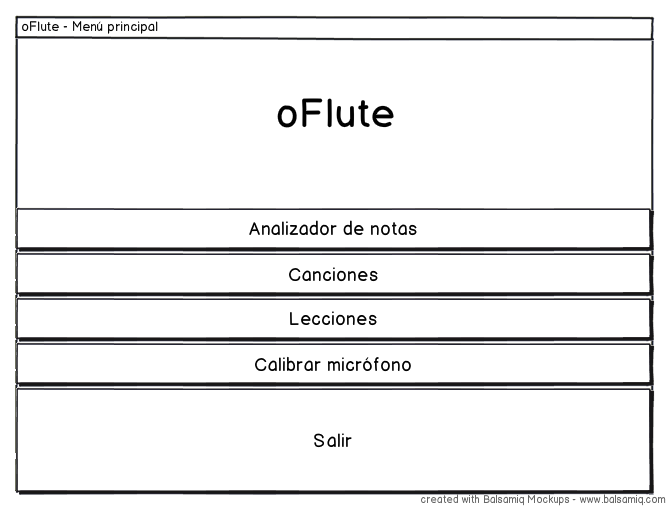
\includegraphics[width=0.9\textwidth]{desarrollo/mockup_menu_principal}
  \caption{Maqueta del menú principal}
\end{figure}


\subsection{Requisitos funcionales}

\subsection{Requisitos de rendimiento}

\subsection{Requisitos de diseño}

\subsection{Requisitos del sistema software}

\section{Modelo de casos de uso}

